\chapter{Extending Peptizer}
%
\section{Introduction}
\npar Upon inspecting MS/MS identification results, a critical scientist has certain \textbf{expectations}. Some of these are automatically used by the database search algorithm to identify an MS/MS spectrum while others are not applicable on a large scale and therefore not used. To the first group belong mass differences between fragment ions as these are general and informative for the peptide sequence. Database search algorithms commonly use these as \textbf{robust features} to interpret a MS/MS spectrum. To the second group belong less general features. For example, it is known that proline-containing peptides are more prone to fragment N-terminally to proline upon CID. But, since not every peptide contains a proline database search algorithms cannot use this as a general robust feature. Hence, this type of information can still be used in a \textbf{complementary }level aside the database search algorithm.
\npar The Peptizer platform does just this. If a critical scientist has certain expectations for his or her MS/MS results, these expectations can be translated into \textbf{custom Agents}. Moreover, the methodology to group these expectations can be translated into a custom \textbf{AgentAggregator}. Both suggest extending Peptizer \textbf{to automate the inspections of a critical scientist's expectations}.
\npar This chapter explains how to extend Peptizer by creating custom Agents and AgentAggregators.
%
\section{Overview}
\npar Both the Agent and the AgentAggregator have a basic \textbf{input output }operation. This is illustrated by the figures below.


%%%%%%
\begin{figure}[H]
\begin{center}
	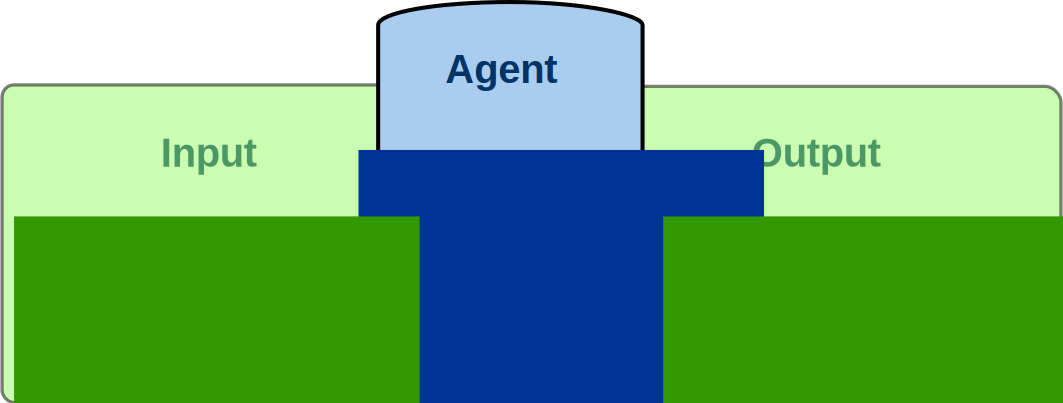
\includegraphics[width=.85\textwidth]{agent_concept}
	\caption{\label{agent_concept} The basic input/output structure of an Agent. As input, the Agent receives a PeptideIdentification object that consists of a single MS/MS spectrum and a number of peptides hypothesises suggested for that spectrum. After this input has been processed by an Agent, a vote is casted as output. This vote refelcts the Agent's opinion for selecting or not selecting the given peptide identification.}
\end{center}
\end{figure}
%


%%%%%%
\begin{figure}[H]
\begin{center}
	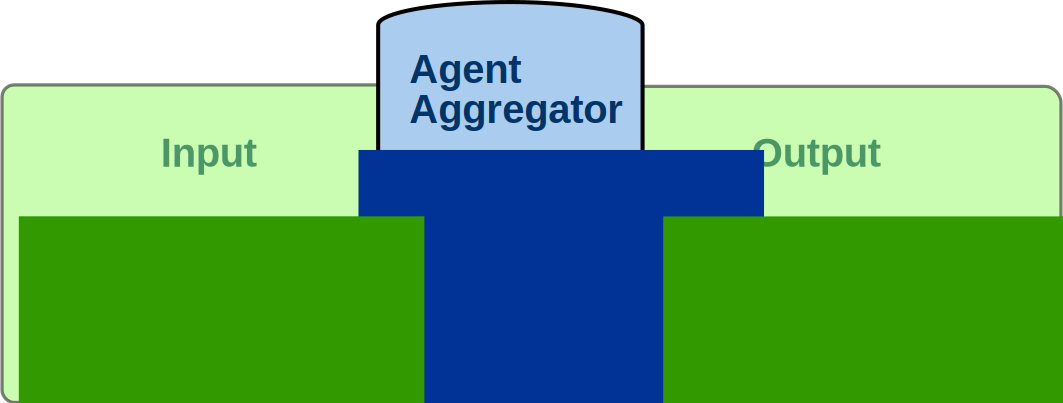
\includegraphics[width=.85\textwidth]{agentaggregator_concept}
	\caption{\label{agentaggregator_concept} The basic input/output structure of an AgentAggregator. As input, the AgentAggregator receives a collection of Agent votes. Therein, \textit{i} Agents vote for selection of a peptide identification, \textit{j} Agents vote neutral for selection while \textit{k} Agents vote against selection. The Agent agregator then processes all votes and concludes as output whether or not the peptide identification is matching and should therefore be selected or not.}
\end{center}
\end{figure}
%
\npar This concept must be kept in mind when extending Peptizer. Next up are instructions for creating an \textbf{easy Agent} followed by a \textbf{more complex Agent}. Finally, the creation of an\textbf{ easy AgentAggregator }is instructed as well.

\section{Writing the first Agent}
\npar For the easy example, a length Agent will be made. Its aim is to \textbf{verify whether a peptide's length is shorter or longer then a given threshold length}. The Agent could then for example be used to select short peptides as these are more prone to generate false positive peptide identifications.
\npar \textit{First} and most important: each custom Agent must \textbf{extend the abstract Agent class}. Thereby, each Agent has \textbf{common variables} and a \textbf{common signature}. Examples for common variables are a name, a status for both the activity and the veto option as well as a common method to get a unique identifier.
\npar \textit{Second}, to set an Agent's variables from the agent.xml configuration file, an Agent must be \textbf{initialized}. After being initialized, an Agent can then receive input and produce output. The initialization is also the place to define \textbf{custom parameters} like the threshold length in this example. This is illustrated in the code snapshot below. There, the value of the LENGTH variable is used to get the appropriate value from the agent.xml configuration file.

%
%
%%%%%
%CODE%
%%%%%
\begin{algorithm}[H]
\caption{Constructing an Agent}
\scriptsize
\vspace{0.3cm}
\begin{verbatim}
public class LengthAgent extends Agent {

   public static final String LENGTH = "length";
	
   public LengthAgent(){
      initialize(LENGTH);
   }
}
\end{verbatim}
\end{algorithm}
%

\npar \textit{Third}, the \textbf{inspect method }must be implemented from the abstract Agent class. This method reflects the basic input/output structure of an Agent: \textbf{a PeptideIdentification object is an input parameter} and \textbf{an array of AgentVotes is returned as output} (one for each peptide hypothesis from the MS/MS spectrum). Note that the different votes are static by on the \textbf{AgentVote enum}.

\npar The inspect method for the LengthAgent can be seen as following. Get the length threshold as a local variable from a Properties object that was created during initialization of the Agent. Then create an array to fit n Agentvotes where n equals the number of confident peptide hypothesises made for the MS/MS spectrum (so we decide to only inspect on confident peptide hypothesises). Then an AgentReport is created  for each of these peptide hypothesesis, wherein results are persisted.
\npar If the length of the peptide sequence is less then the length threshold, the LengthAgent votes positive for selection. Else it votes neutral for selection. Finaly, the reports are made and stored along the PeptideIdentification. These reports are used to display the PeptideIdentification in the Peptizer graphical user interface.

%
%
%%%%%
%CODE%
%%%%%
\begin{algorithm}[H]
\caption{Inspect method of the Length Agent}
\scriptsize
\vspace{0.3cm}
\begin{verbatim}
public AgentVote[] inspect(PeptideIdentification aPeptideIdentification) {

        int lLength = Integer.parseInt((String) (this.iProperties.get(LENGTH)));
        AgentVote[] lVotes = new AgentVote[aPeptideIdentification.getNumberOfConfidentPeptideHits()];

        for (int i = 0; i < lVotes.length; i++) {

	    	PeptideHit lPeptideHit = aPeptideIdentification.getPeptideHit(i);
	   		AgentReport lReport = new AgentReport(getUniqueID());

            int lPeptideLength = lPeptideHit.getSequence().length();

            if (lPeptideLength < lLength) {
                lVotes[i] = AgentVote.POSITIVE_FOR_SELECTION;
            } else {
                lVotes[i] = AgentVote.NEUTRAL_FOR_SELECTION;
            }

            lReport.addReport(AgentReport.RK_RESULT, lVotes[i]);
            lReport.addReport(AgentReport.RK_TABLEDATA, new Integer(lPeptideLength));
            lReport.addReport(AgentReport.RK_ARFF, new Integer(lPeptideLength));

            aPeptideIdentification.addAgentReport(i + 1, getUniqueID(), lReport);
        }
        return lVotes;
    }
\end{verbatim}
\end{algorithm}
%


\npar In the end, the LengthAgent returns an Agentvote for each confident peptide hypotheseis. Whereas each vote reflects the length of the peptide in relation to the given length threshold.
\npar After this easy example, lets create an Agent with more advance processing features.

\section{A more advanced Agent}

\subsection{Background}
This section starts with a quote from a 2004 paper by Ross et al.:
\begin{quote}
\textsf{We have developed a multiplexed set of reagents for quantitative protein analysis that place isobaric mass labels at the N termini and lysine side chains of peptides in a digest mixture. The reagents are differentially isotopically labelled such that all derivatized peptides are isobaric and chromatographically indistinguishable, but yield signature or reporter ions following CID that can be used to identify and quantify individual members of the multiplex set.}
\newline
\footnotesize Ross, P. L. et al. (2004). "Multiplexed protein quantitation in Saccharomyces cerevisiae using amine-reactive isobaric tagging reagents." Mol Cell Proteomics 3(12): 1154-69.
 \end{quote}
 \npar Ross et al. introduced the \ITRAQ methodology that has become a widespread tool for quantitative proteomics. If this chemistry is used, then \ITRAQ reporter ions are expected to appear in the MS/MS spectrum. If these reporter ions appear in unequal intensities, then the corresponding peptide was differentially abundant in both samples.
 \npar This can now be defined as a case to create a new Agent:\\{\textbf{Do \ITRAQ reporter ions appear at different intensity?}
%
%SECTION
\subsection{Creating a custom Agent to inspect expectations}
 \npar A custom Agent inspecting the appearance of \ITRAQ reporter ions in the MS/MS spectrum will now be created. This Agent will be named as the ReporterIonAgent. Just as any other Agent in Peptizer, the ReporterIonAgent must extend the abstract Class Agent. This abstract class has common methods and variables among all Agents.\footnote{Read more on abstract classes at \url{http://java.sun.com/docs/books/tutorial/java/IandI/abstract.html}} Examples of common features are the name, the activity or the veto status as well as the getters and the setters to modify these variables. As such, the ReporterIonAgent must only encode its differences from other Agents.
\npar A custom Agent like the ReporterIonAgent can be created from \textbf{the template signature of an Agent extension}. This template is availlable as the \textbf{DummyAgent} in the standard Peptizer distribution.\footnote{The DummyAgent can be found in the Peptizer package be.proteomics.mat.util.agents. Click to browse the \href{http://genesis.ugent.be/peptizer/xref/be/proteomics/mat/util/agents/DummyAgent.html}{Java source code} or the \href{http://genesis.ugent.be/peptizer/apidocs/be/proteomics/mat/util/agents/DummyAgent.html}{JavaDocs} on this DummyAgent template to create custom Agents.}
\begin{description}
\item[Parameters] Declare optional parameters that are used as options by this Agent.\\\textit{The mass over charge values for reporter ions}
\item[Constructor] Declare the instantiation method of an Agent extension.\\\textit{The initiation of the super class Agent and the set-up of the private variables of ReporterIonAgent}
\item[Inspection] Define the inspection logic that the Agent must perform.\\\textit{The inspection of the Agent reports whether ITRAQ reporter ions appear at different intensities}
\item[Description] Document the aim of this Agent.
 \end{description} 
 \npar These elements are illustrated by the DummyAgent in the following Java code snippet.
%
%
%%%%%
%CODE%
%%%%%
\begin{algorithm}[H]
\caption{Agent signature in a code outline}
\scriptsize
\vspace{0.3cm}
\begin{verbatim}
public class DummyAgent extends Agent {

   //Parameters
   public static final String DUMMY_PROPERTY = "dummy";
	
   //Constructor
   public DummyAgent(){
      super();
      ...
   }
	
   //Inspection
   public AgentVote[] inspect(PeptideIdentification aPeptideIdentification){
      AgentVote vote = null;
      ...
      return vote;
   }
	
   //Description
   public String getDescription(){
      return "Agent description";
   }
}
\end{verbatim}
\end{algorithm}
%
\npar Ok, so now being aware of the code signature of an Agent, the ReporterIonAgent can be created similarly.
\subsubsection{PARAMETERS}
\npar First, the different \textbf{parameters} required by this Agent must be defined. Since these are read from the configuration file, they must have fixed identifiers. There are two parameters holding the values for the two \textbf{reporter ion masses} and a \textbf{fold ratio threshold} between the two reporter ion intensities for this Agent to inspect. Finally, there is also a parameter on the \textbf{error tolerance} that is allowed upon matching the reporter ion masses with a fragment ion from the MS/MS spectrum.
\npar In Java, each of these is encoded as final static Strings, since these are then always \textbf{identical }and \textbf{accessible}.
\npar The parameters for the ReporterIonAgent are illustrated in the following Java code snippet.
%
%
%%%%%
%CODE%
%%%%%
\begin{algorithm}[H]
\caption{Parameters for the ReporterIonAgent}
\scriptsize
\vspace{0.3cm}
\begin{verbatim}
   //Mass over charge value for the first reporter ion.
   public static final String MASS_1 = "reporter_mz_1";

   //Mass over charge value for the second reporter ion.
   public static final String MASS_2 = "reporter_mz_2";

   //Fold ratio between the two reporter ions. 
   public static final String RATIO = "ratio";

   //Error tolerance for matching the expected
   //reporter ion mass over charge to a fragment ion.
   public static final String ERROR = "error";
\end{verbatim}
\end{algorithm}
%
%
\npar Ok, after defining the parameters, the code for constructing the Agent can be written.
\subsubsection{CONSTRUCTOR}
\npar The constructor is a special kind of routine as it is only once used upon starting a new Java object. The following parts can be recognized in the code:
\begin{description}
\item[Call superclass constructor] to initiate all methods and variables common to all Agents at their superclass.
\item[Read properties] from the agent.xml configuration file for the Agent with this unique identifier. 
\item[Set general variables] as given by the agent.xml configuration file to general agent variables like the name, the active and the veto status.
\item[Set specific variables] as given by the agent.xml configuration file to specific agent variables like the reporter ion masses, the ratio and the error tolerance.\\Note that this is enclosed by a try \& catch statement. If these variables are not inside the configuration file, then Peptizer will log an exceptional GUI message before shutting down the application.
\end{description}
\npar The construction of the ReporterIonAgent is illustrated in the following Java code snippet:
%
%%%%%
%CODE%
%%%%%
\begin{algorithm}[H]
\caption{Construction of an Agent}
\scriptsize
\vspace{0.3cm}
\begin{verbatim}
   /**
   * Construct a new instance of the ReporterIonAgent.
   */
   public ReporterIonAgent() {

      super();
      Properties prop = MatConfig.getInstance().getAgentProperties(this.getUniqueID());
      super.setName(prop.getProperty("name"));
      super.setActive(Boolean.valueOf(prop.getProperty("active")));
      super.setVeto(Boolean.valueOf(prop.getProperty("veto")));

      try {

         this.iProperties.put(MASS_1, prop.getProperty(MASS_1));
         this.iProperties.put(MASS_2, prop.getProperty(MASS_2));
         this.iProperties.put(RATIO, prop.getProperty(RATIO));
         this.iProperties.put(ERROR, prop.getProperty(ERROR));

      } catch (NullPointerException npe) {

         MatLogger.logExceptionalGUIMessage(
         "Missing Parameter!!", "Parameters " + MASS_1 + ", " + MASS_2 + " , " +
         RATIO + "and "+ ERROR + " are required! for Agent " + this.getName() +
         " !!\nExiting..");
         
         System.exit(0);
   }
}
\end{verbatim}
\end{algorithm}
\npar With all this information, the ReporterIonAgent is ready to inspect an MS/MS spectrum for its reporter ions.
\subsubsection{INSPECTION}
\npar The inspection is the core of an Agent since this logic leads to the Agent's vote. The \textbf{input }of the inspection is a PeptideIdentifcation object. Such an object has a single MS/MS spectrum and multiple peptide hypothesises. The \textbf{output} of the inspection is a vote as an AgentVote enumeration. There are three types of votes:
\begin{enumerate}
\item A vote approving to select the peptide hypothesis for a given property.\\\textit{Peptide hypothesises of MS/MS spectra with deviating reporter ion intensities}
\item A vote being neutral to select the peptide hypothesis for a given property.\\\textit{Peptide hypothesises from MS/MS spectra with equal reporter ion intensities}
\item A vote denying to select the peptide hypothesis for a given property.\\\textit{Peptide hypothesises from MS/MS spectra lacking reporter ion fragment ions}
\end{enumerate}
\npar Note that examples for the ReporterIonAgent shown in \textit{italics} depend on expectations of the scenario, on what peptide hypothesises are interesting to the case that is initially defined. Therefore it is very important to document the Agents in depth.
%
\npar This ReporterIonAgent is documented exhaustively so it is possible to read through to code step by step. As such, the source code of the ReporterIonAgent is included below. Comments are formatted in grey italics while Java keywords are blue and text values are green. The inspection part of the code starts from line 82. From thereon, the following parts can be recognized: 
\begin{description}
\item[Preparing the variables (line 109)] Here, a set of variables are defined that are needed to perform the inspection.\\\textit{Variables to hold the observed peak intensity or matching status.}
\item[Inspecting for the reporter ions(line 145)] Here, the actual inspection is performed.\\\textit{Finding the reporter ions in the MS/MS spectrum, calculate their intensity ratio and test if it meets the expectations.}
\item[Making an inspection report and committing the votes(line 236)] Here, the results of the inspection are stored and returned as an AgentVote for each peptide hypothesis.\\\textit{Store the intensity ratio and the votes in a report that will be read by the AgentAggregator.}
\end{description}
%
%% IntelliJ print options:
% Gentium basic, 10pt, Line numbers, Color printing, Syntax printing.
% Header left, Gentium Basic bold, 12pt
% Wrap at word breaks, Top 1.0, Left 1.0, Right 1.0, Bottom 0.7
%
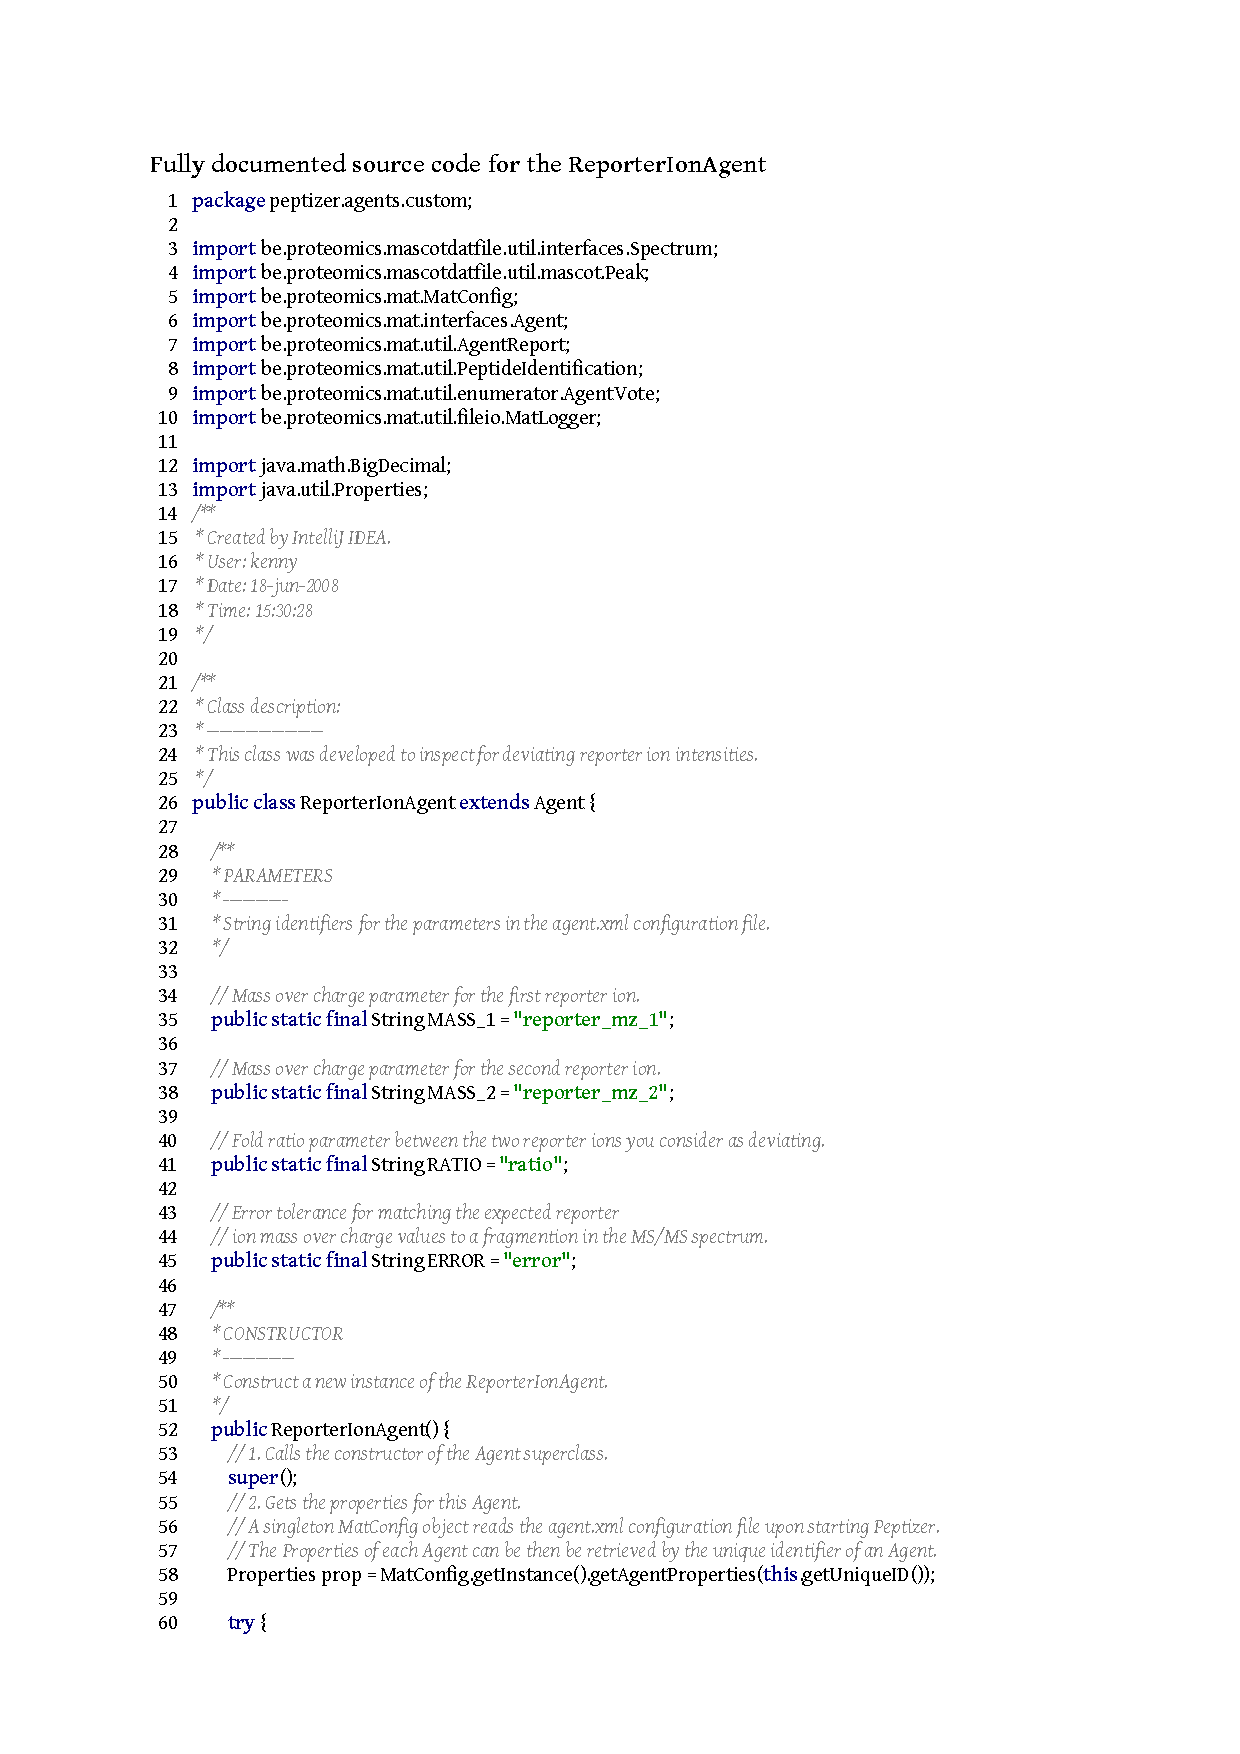
\includepdf[pages={1-5}]{reporterionagent_source.pdf}
\subsubsection{DESCRIPTION}
\npar The final method that must be implemented for each Agent is a descriptive method. Here resides the hard coded description the user reads in the Agent table upon starting a new Peptizer selection task. In addition, when the user is validating a Peptide hypothesis this description shows up in the information table.
\npar It is important to stress shortly what it does, but also how an Agent casts a vote.
%
%%%%%
%CODE%
%%%%%
\begin{algorithm}[H]
\caption{Agent description}
\scriptsize
\vspace{0.3cm}
\begin{verbatim}
   /**
   * Describe the ReporterIonAgent shortly.
   */
   public String getDescription() {
   return "<html>Inspects for the abberant reporter ion intensities." +
               "<b>Selects when two reporter ions ( " + this.iProperties.get(MASS_1) +
               " , " + this.iProperties.get(MASS_2) + ") have a more then " +this.iProperties.get(RATIO) +
               " fold intensity ratio.";
   }
\end{verbatim}
\end{algorithm}
\section{Using a custom Agent in Peptizer}
\npar The custom ReporterIonAgent is ready to be used in Peptizer. Therefore, the ReporterIonAgent must be added to the agent configuration file. This includes information on the classpath and classname as well as the Agent's parameters (see \ref{configuration_files} for more information on the configuration files). This looks as following:
%
\begin{verbatim}
<agent>
		<uniqueid>peptizer.agents.custom</uniqueid>
		<property name="name">Reporter Ion Agent</property>
		<property name="active">true</property>
		<property name="veto">false</property>
		<property name="reporter_mz_1">114.1</property>
		<property name="reporter_mz_2">117.1</property>
		<property name="ratio">1.5</property>
		<property name="error">0.2</property>		
</agent>
\end{verbatim}
\npar When a new selection task is started , the ReporterIonAgent is availlable to inspect peptide hypothesises as illustrated below.
%
%%%%%%
%FIGURE%
%%%%%%
\begin{figure}[H]
\begin{center}
	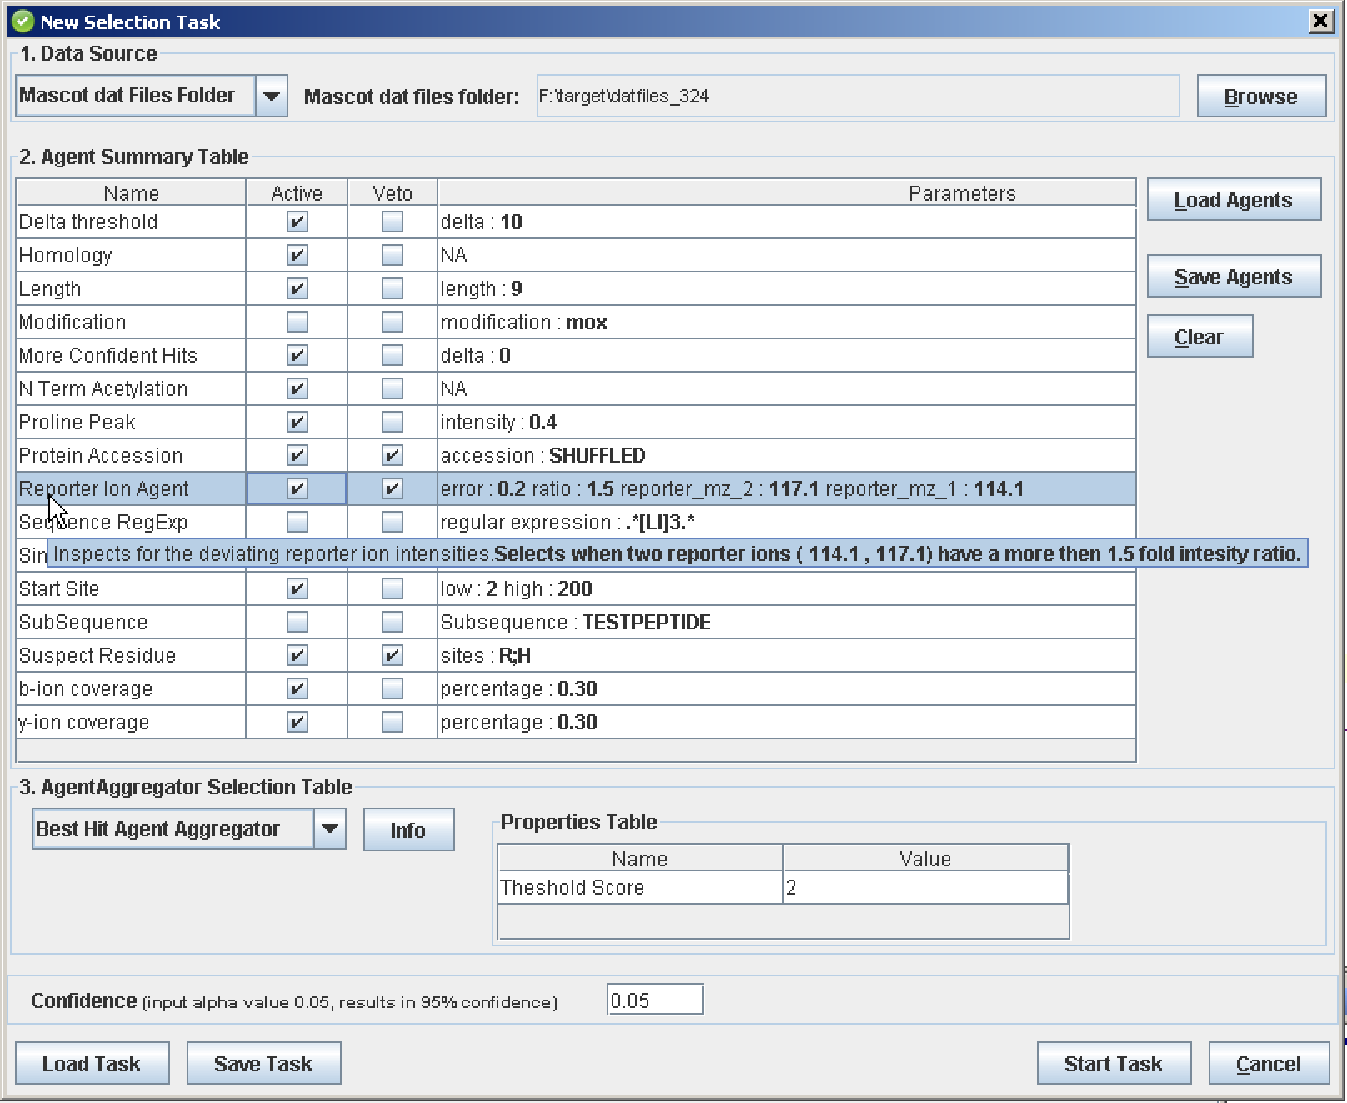
\includegraphics[width=.85\textwidth]{reporterion_task}
	\caption{\label{reporterion_task}After adding the ReporterIon Agent to the agent configuration file, the ReporterIon Agent can be used for creating a new Peptizer task.}
\end{center}
\end{figure}
%
\npar Peptizer will then inspect each MS/MS spectrum for deviating reporter ion intensities by using the ReporterIon Agent. As such, peptide hypothesises originating from MS/MS spectra with deviating reporter ion intensities will be selected and shown in the manual validation GUI of Peptizer. This is shown in the figure below. Note that this list can also be saved as a comma separated file (see \ref{save_csv_txt}).
%
%%%%%%
%FIGURE%
%%%%%%
\begin{figure}[H]
\begin{center}
	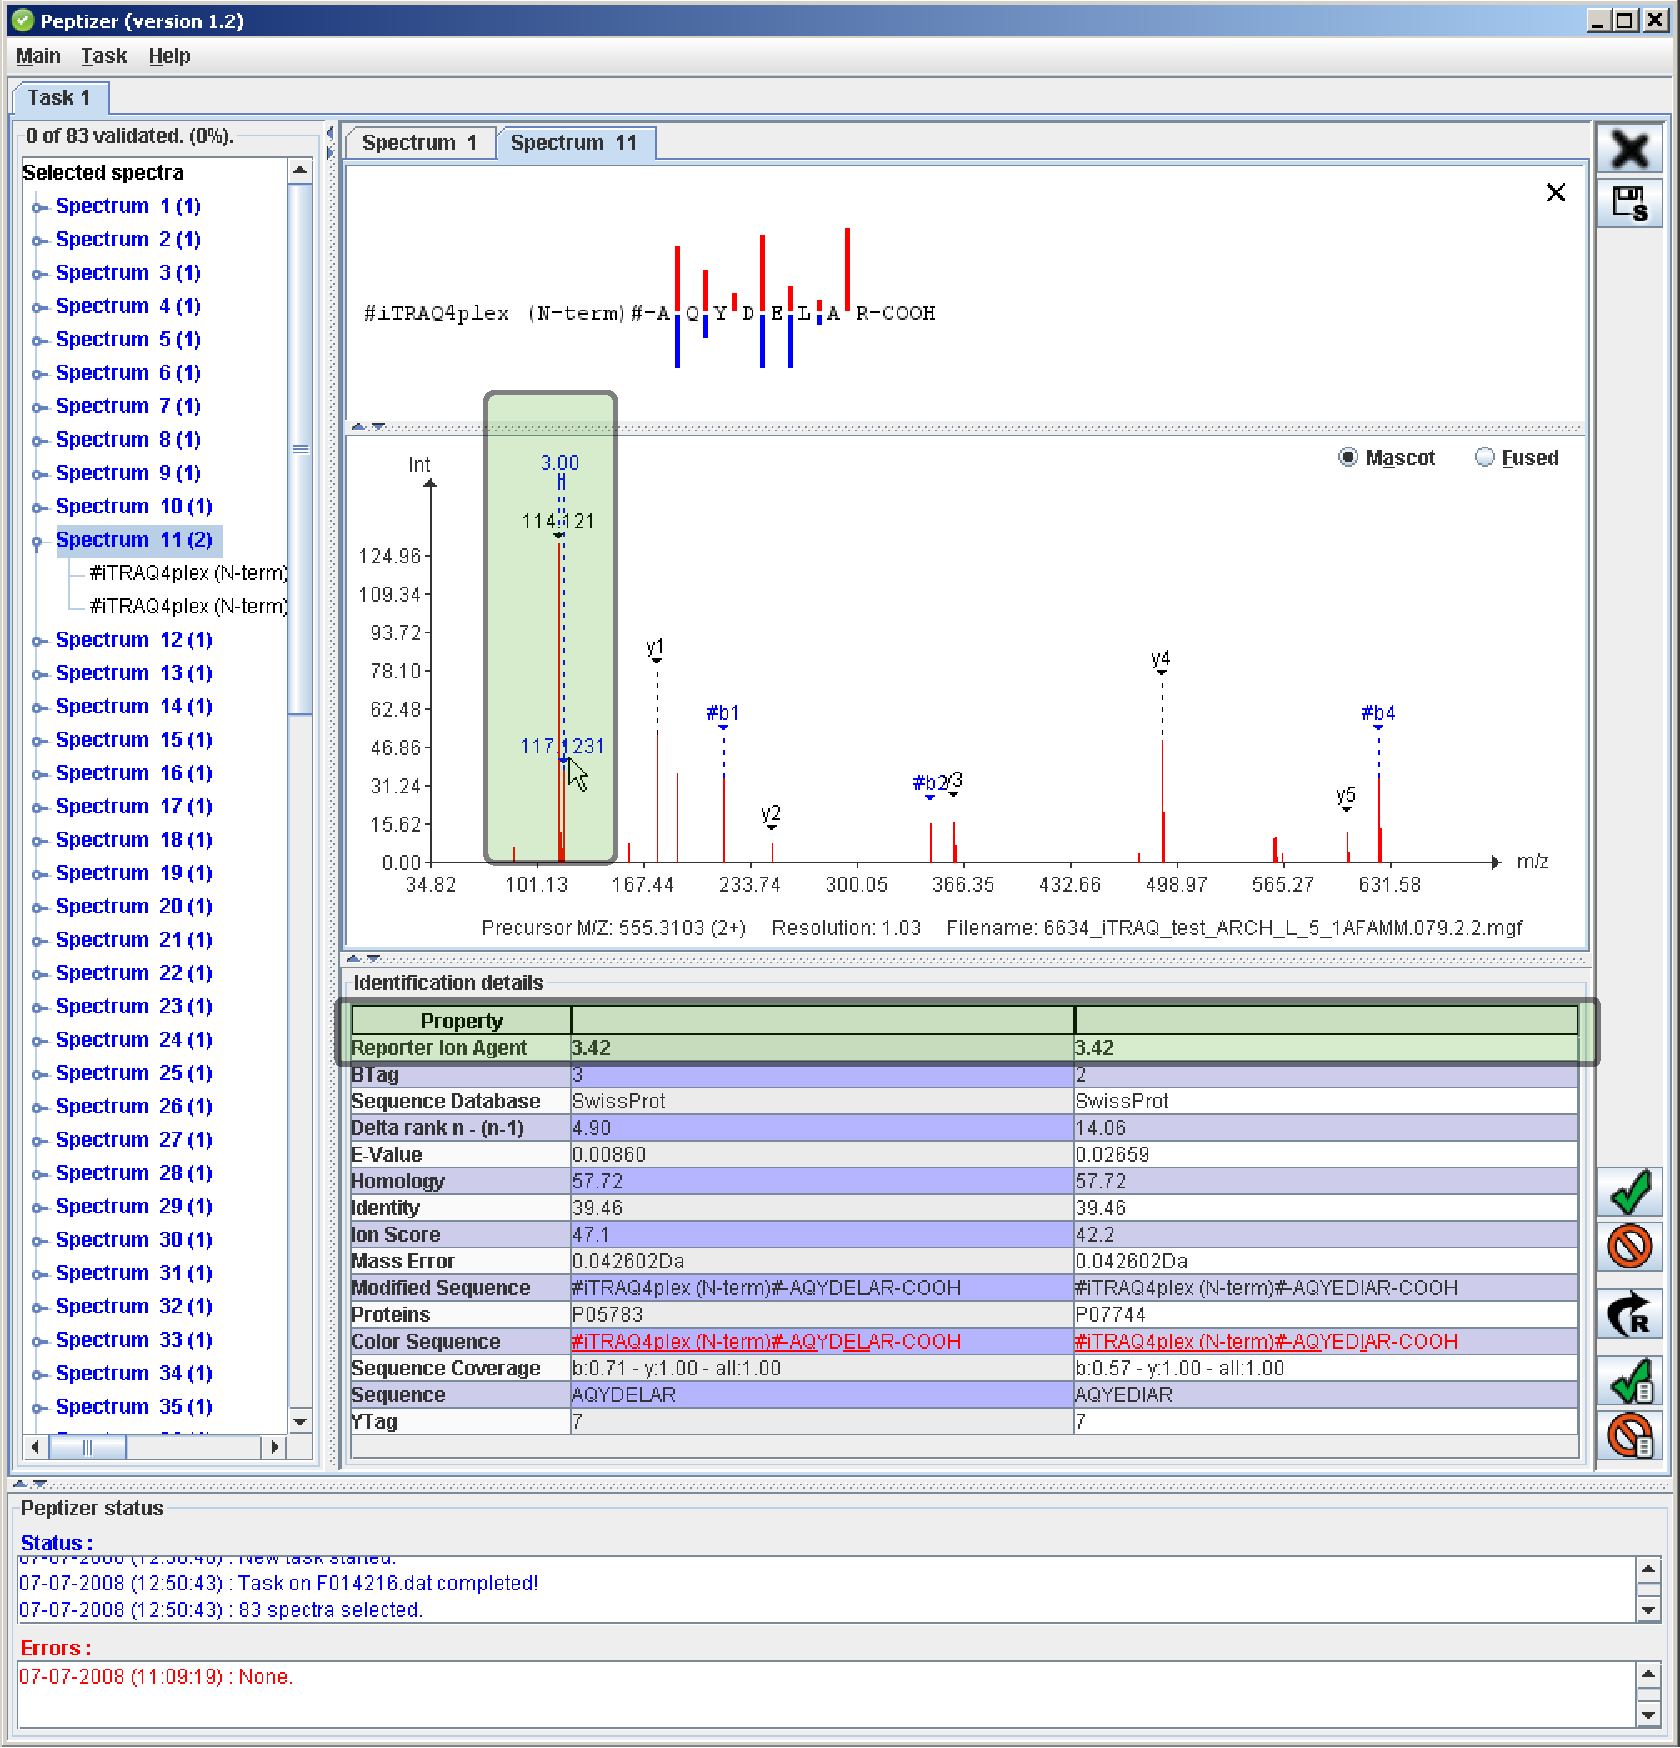
\includegraphics[width=.85\textwidth]{reporterion_validation}
	\caption{\label{reporterion_task}By using the ReporterIon Agent, Peptizer selected all peptide hypothesises from MS/MS spectra with deviating reporter ion intensities. Both green boxes show how the ReporterIon Agent first identifies the reporter ions in the MS/MS spectrum and used these to calculate the intensity ratio of \textbf{3.42}. Since this is more then the threshold ratio that was set to \textbf{1.5}, this peptide hypothesis was selected for its deviating reporter ion intesities in the MS/MS spectrum.}
\end{center}
\end{figure}
%
\section{Writing your own AgentAggregator}

\npar Finally, when a series of Agents voted on a MS/MS spectrum and it's peptide hypothesises, these \textbf{Agent votes are input for an AgentAggregator}. The task of an AgentAggregator is then to bundle these votes and produce a conclusion whether or not the a PeptideIdentification matches a profile defined by its Agents.
\npar The BestHitAggregator serves as an example for creating a custom AgentAggregator. The construction of a AgentAggregator is very similar to that of an Agent. First, all AgentAggregators must \textbf{extend the abstract AgentAggregator class} so to have a common set of variables and a \textbf{common signature}. Second, an AgentAggregator must also be \textbf{initialized} to set its properties from the aggregator.xml configuration file.

%
%
%%%%%
%CODE%
%%%%%
\begin{algorithm}[H]
\caption{AgentAggregator construction}
\scriptsize
\vspace{0.3cm}
\begin{verbatim}
public class BestHitAggregator extends AgentAggregator {
    public static final String SCORE = "score";

    public BestHitAggregator() {
        initialize(SCORE);
    }
\end{verbatim}
\end{algorithm}
%

\npar Also like in the Agent, the input/output structure of the AgentAggregator makes sense upon \textbf{implementing the abstract match method }from the AgentAggregator class. Again, a \textbf{PeptideIdentification object serves as an input parameter }and \textbf{a single AgentAggregatorResult is returned as output}. Note that the different aggregation results are static on the AgentAggregatorResult enum.

\npar A collection of Agents is set upon starting a Peptizer task on the abstract AgentAggregator class. Therefore, an AgentAggregator implementation has no concern on the type of Agents, it must only be aware that there are some Agents ready for voting.

\npar \textit{First}, a number of local variables are declared that are used during the routine. Then, there is a check if there is any confident peptide hypothesis for this MS/MS spectrum. Only then starts \textbf{an iteration over all the availlable Agents}. Each Agent then \textbf{inspects the PeptideIdentification and returns an AgentVote}. As this is the BestHitAggregator, \textbf{only the votes for the best peptide hypothesis are taken into consideration here}. During iteration, the veto status of an Agent is also logged, but only if the Agent is positive for selection.

%
%%%%%
%CODE%
%%%%%
\begin{algorithm}[H]
\caption{BestHitAggregator matching method}
\scriptsize
\vspace{0.3cm}
\begin{verbatim}
    public AgentAggregationResult match(PeptideIdentification aPeptideIdentification) {

        boolean boolConfident = false;
        boolean boolMatch = false;
        boolean boolVetoWasCalled = false;

        Integer lThresholdScore = new Integer(iProperties.getProperty(SCORE));

        int counter = -1;
        AgentVote[] results = new AgentVote[iAgentsCollection.size()];

        if (aPeptideIdentification.getNumberOfConfidentPeptideHits() > 0) {
            boolConfident = true;
            for (Agent lAgent : iAgentsCollection) {
                
                counter++;

                results[counter] = lAgent.inspect(aPeptideIdentification)[0];
                if (results[counter] == AgentVote.POSITIVE_FOR_SELECTION && lAgent.hasVeto()) {
                    boolVetoWasCalled = true;
                }
            }

           if (boolVetoWasCalled) {
                boolMatch = true;
            } else {
                int lSumScore = sumVotes(results);

                if (lSumScore >= lThresholdScore) {
                    boolMatch = true;
                }
            }

        }

        if (boolConfident) {
            if (boolMatch) {
                return AgentAggregationResult.MATCH;
            } else {
                return AgentAggregationResult.NON_MATCH;
            }
        } else {
            return AgentAggregationResult.NON_CONFIDENT;
        }
    }
\end{verbatim}
\end{algorithm}
%
\npar When the iteration has finished, a few lines of logic aggregate the votes. \textit{First}, if an Agent with veto rights was positive for selection then it is a match for sure. \textit{Second}, all votes are summed and compared with the scoring threshold as given by the user. If the sum is greater then the threshold, then it is a match. Else, a PeptideIdentification is not matched or not confident. The AgentAggregator concludes by returning a corresponding AgentAggregatorResult object.

\npar In the end, the BestHitAggregator will thus have returned a conclusion on a given PeptideIdentification. Those PeptideIdentifications with a \textbf{AgentAggregatorResult.MATCH} result are subsequently presented in the \textbf{manual validation interface} of Peptizer.